\documentclass{article}
\usepackage{covington}
\usepackage{comment}
\usepackage{url}
\usepackage{mathtools}
\usepackage{tipa}
\usepackage[UKenglish]{babel}
\usepackage{graphicx}
\usepackage{subfigure}
%\usepackage{savetrees}
\usepackage[margin=1.0in]{geometry}


% Default fixed font does not support bold face
\DeclareFixedFont{\ttb}{T1}{txtt}{bx}{n}{8} % for bold
\DeclareFixedFont{\ttm}{T1}{txtt}{m}{n}{8}  % for normal

% Custom colors
\usepackage{color}
\definecolor{deepblue}{rgb}{0,0,0.5}
\definecolor{deepred}{rgb}{0.6,0,0}
\definecolor{deepgreen}{rgb}{0,0.5,0}

\usepackage{listings}
\lstset{
language=Matlab,
basicstyle=\ttm,
breaklines=true,
otherkeywords={self},             % Add keywords here
keywordstyle=\ttb\color{deepblue},
emph={MyClass,__init__},          % Custom highlighting
emphstyle=\ttb\color{deepred},    % Custom highlighting style
stringstyle=\color{deepgreen},
frame=tb,                         % Any extra options here
showstringspaces=false  
}

\newcommand{\code}[2]{
  \hrulefill
  \subsection*{#1}
  \lstinputlisting{#2}
  \vspace{2em}
}


\begin{document}
\title{AV Assignment 2\\``3D Image Analysis''}
\author{s0949775 and s1330128}
\date{\today}
\maketitle


\section{Introduction}
This report covers the construction of a 3D model from a 
sequence of RGB and depth frames from the Kinect. 
The algorithms we chose and explored are discussed for
each phase of processing:
\begin{itemize}
\item extracting the bin from the RGB images and corresponding 3D points.
\item aligning the extracted bin points from each frame in a single coordinate frame.
\item combining the aligned bit points into a single dataset and fitting two planes.
\end{itemize}

\subsection{Box extraction}
To extract box (figure \ref{fig:extracted_box_example}) we used the fact that it has two orange regions.
We found bottom orange region of the box and then took all of the
pixels above it. After extracting these points from image, we 
intersected them with depth information (figure \ref{fig:full_depth_data_picture}) - we removed part of
pixels that are above top orange region using the fact that above
the box all of the depth values are NaN.

\begin{figure}[h!]
  \centering
  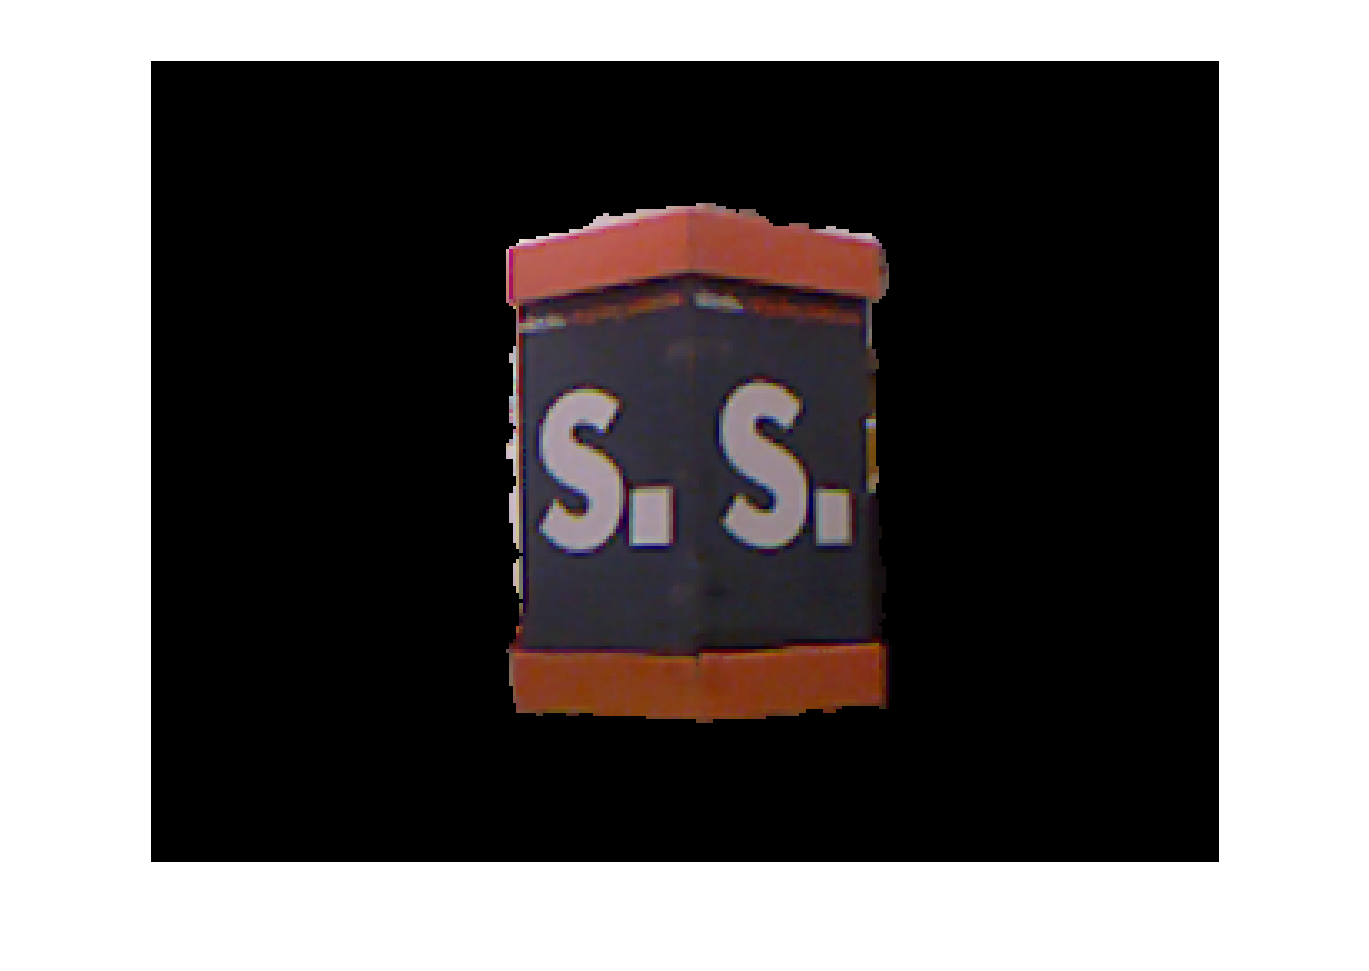
\includegraphics[width=1.0\textwidth]{figs/extracted_box_example}
  \caption{Extracted box example}
  \label{fig:extracted_box_example}
\end{figure}


For actual region lookup, basic color thresholding was used
since orange region had very distinguishable color. Before 
thresholding we converted regular RGB colors
to chromaticity colors (figure \ref{fig:full_chromaticity_image}) to reduce impact of lighting
and applied gaussian smoothing on pixels of
the frame. After these stops two big regions of
orange were found and we took the biggest one
since bottom region is always the biggest (later it 
even gets truncated because box gets out of frame).
Found mask can be seen in figure \ref{fig:detected_bottom_orange_region_mask}.

\begin{figure}[h!]
    \centering
      \subfigure[RGB image converted to chromaticity coordinates]{
        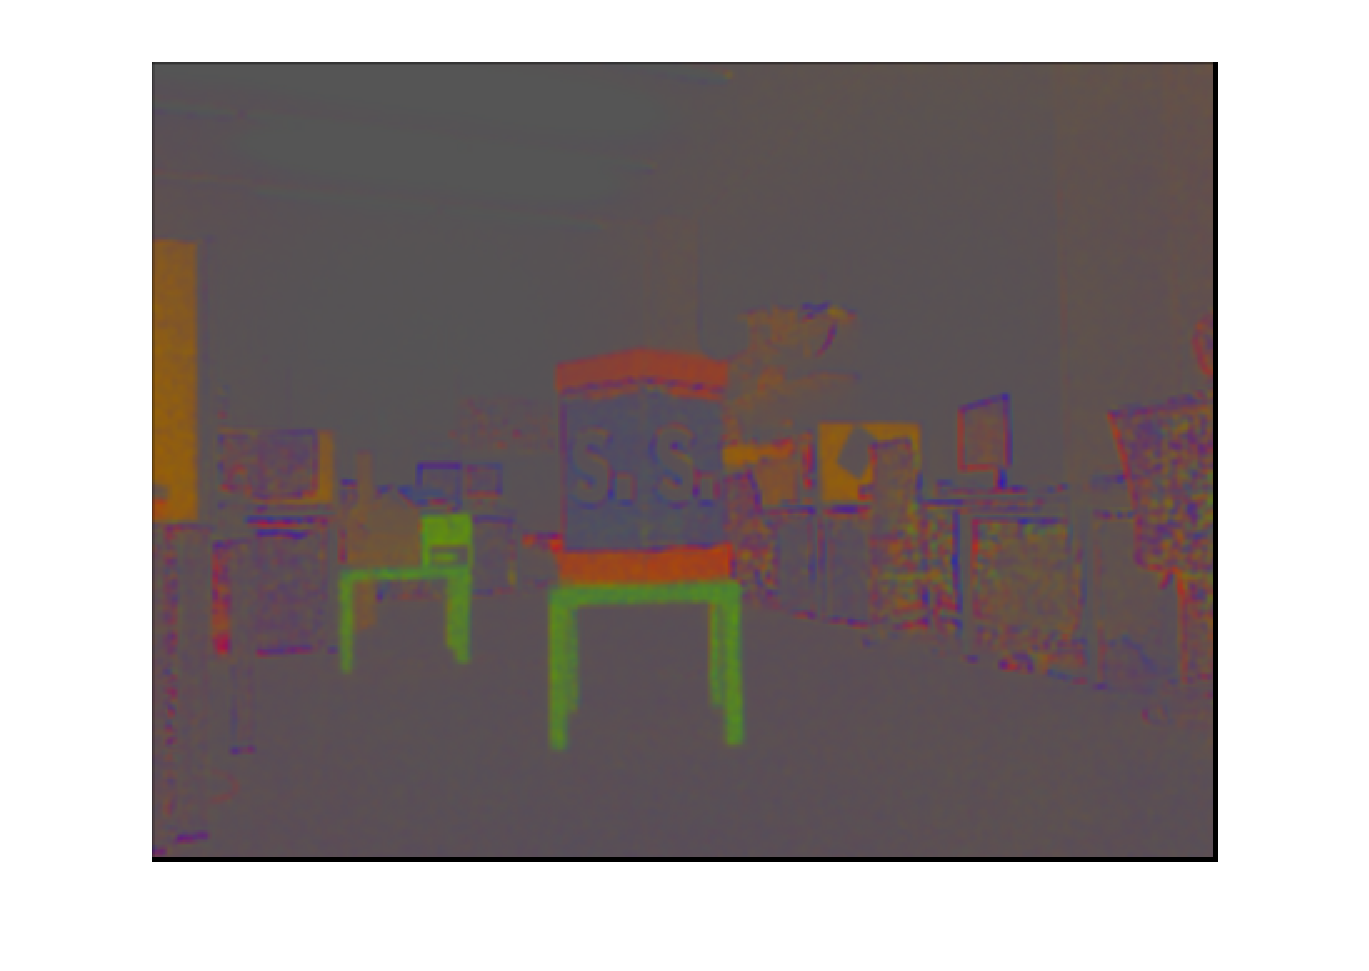
\includegraphics[width=0.4\linewidth]{figs/full_chromaticity_image}
        \label{fig:full_chromaticity_image}
      }
      \subfigure[Depth points of the frame]{
        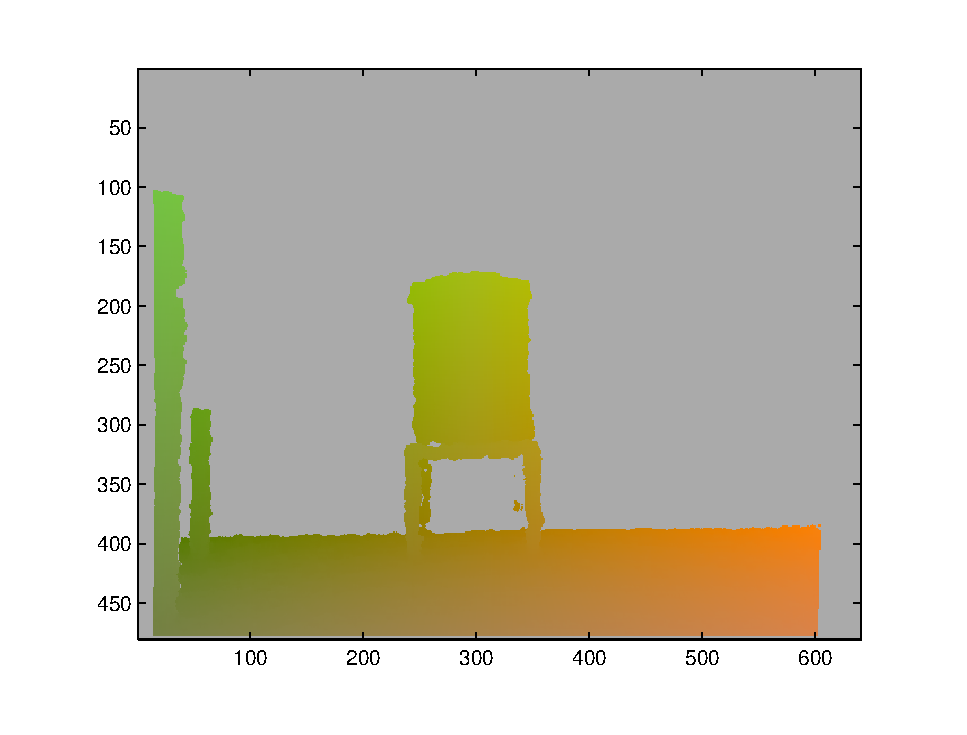
\includegraphics[width=0.4\linewidth]{figs/full_depth_data_picture}
        \label{fig:full_depth_data_picture}
      }
      \quad
      \subfigure[Thresholding colors to find orange regions]{
        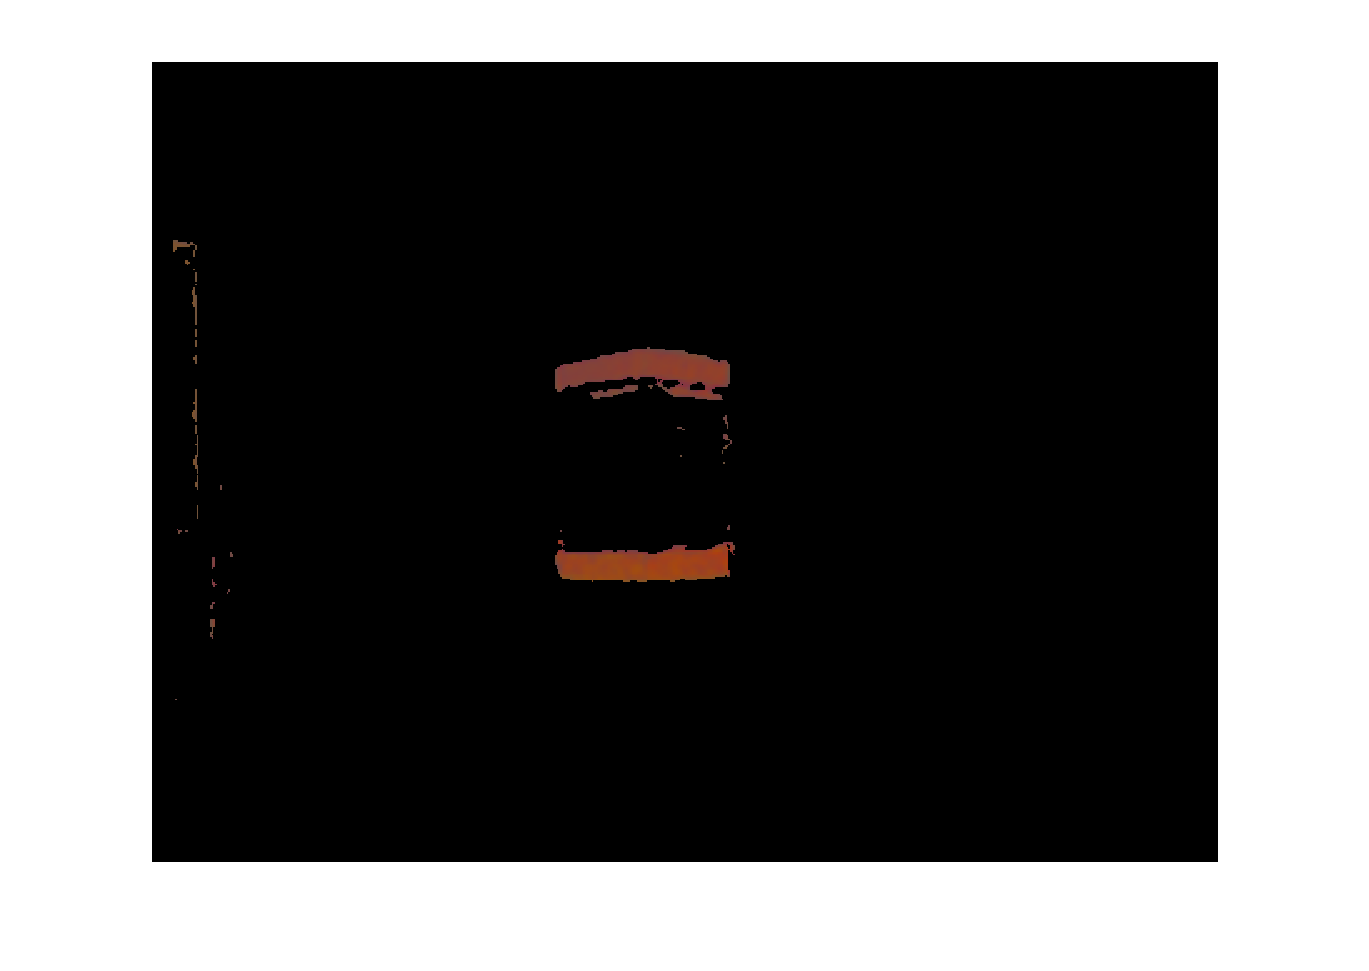
\includegraphics[width=0.4\linewidth]{figs/thresholding_result}
        \label{fig:thresholding_result}
      }
      \subfigure[Detected bottom region mask]{
        \includegraphics[width=0.4\linewidth]{figs/detected_bottom_orange_region_mask}
        \label{fig:detected_bottom_orange_region_mask}
      }
      \caption{Box extraction steps}
\end{figure}

Colours for region thresholding (figure \ref{fig:thresholding_result}) we fine-tuned manually.



\begin{figure}[h!]
    \centering
      \subfigure[Depth point data from single frame]{
        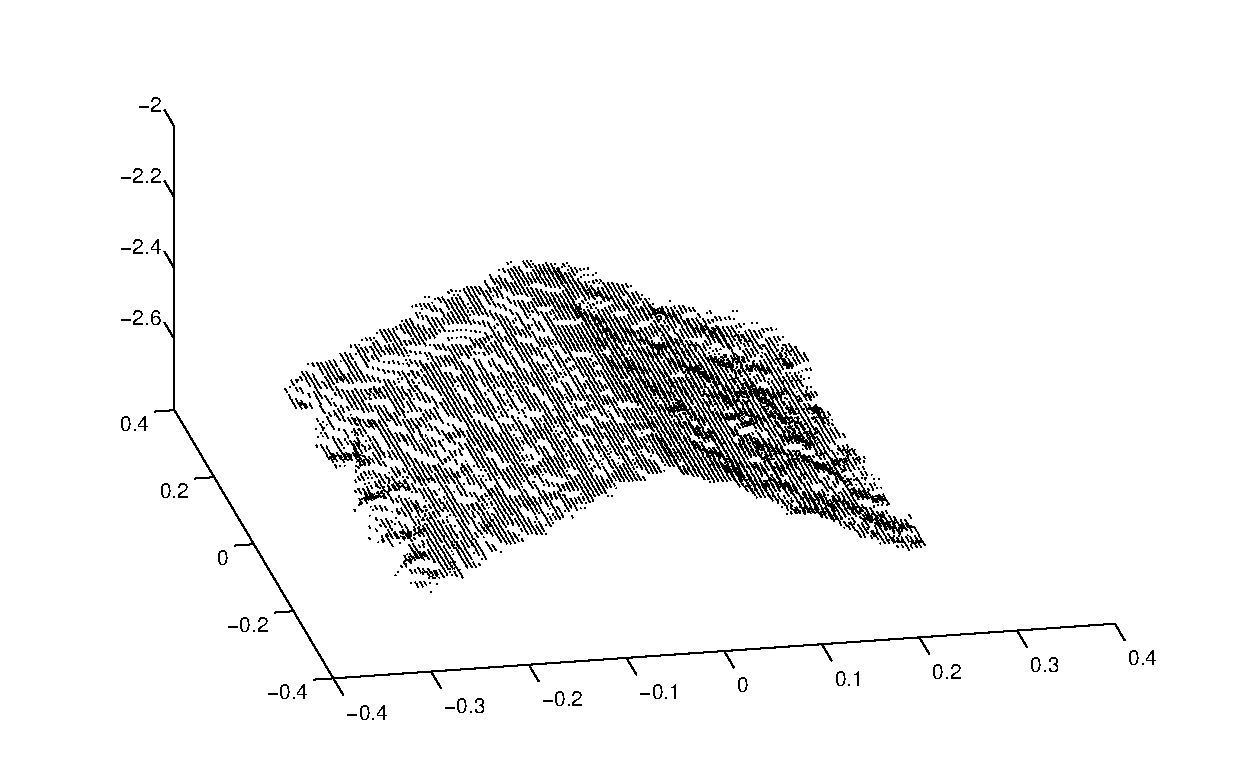
\includegraphics[width=0.4\linewidth]{figs/depth_points_example}
        \label{fig:depth_points_example}
      }
      \subfigure[Coloured depth points]{
        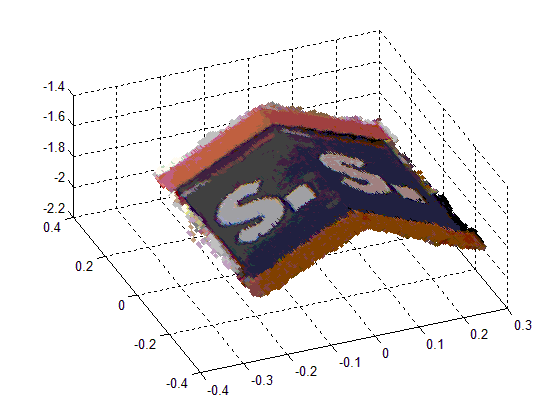
\includegraphics[width=0.4\linewidth]{figs/coloured_depth_points}
        \label{fig:coloured_depth_points}
      }
      \caption{Extracted box examples}
\end{figure}

Extracted coloured 

\subsection{Point alignment}
As was suggested in the assignment we took middle frame
from the sequence as our foundation frame. Against it all
other frame we compared.

To align points for different frames we used ICP algorithm
that was given in the assignment. As actual data that was 
supplied to ICP we used edge points 
(see figure \ref{fig:icp_before_alignment_from_side}
and \ref{fig:icp_before_alignment_from_top}).
 Current box's image
was converted to greyscale and MATLAB's canny was used
to find edges. Using edges, we selected only those
depth points that we under the edges. We tuned edge
detector to detect only long edges that have bigger
intensity changes thus finding few but high quality edges
(can be seen in figure \ref{fig:extracted_edge_mask}).
This allowed ICP to run fast and produce alignments
of high quality (see figure \ref{fig:icp_point_alignment_example}).

\begin{figure}[h!]
  \centering
  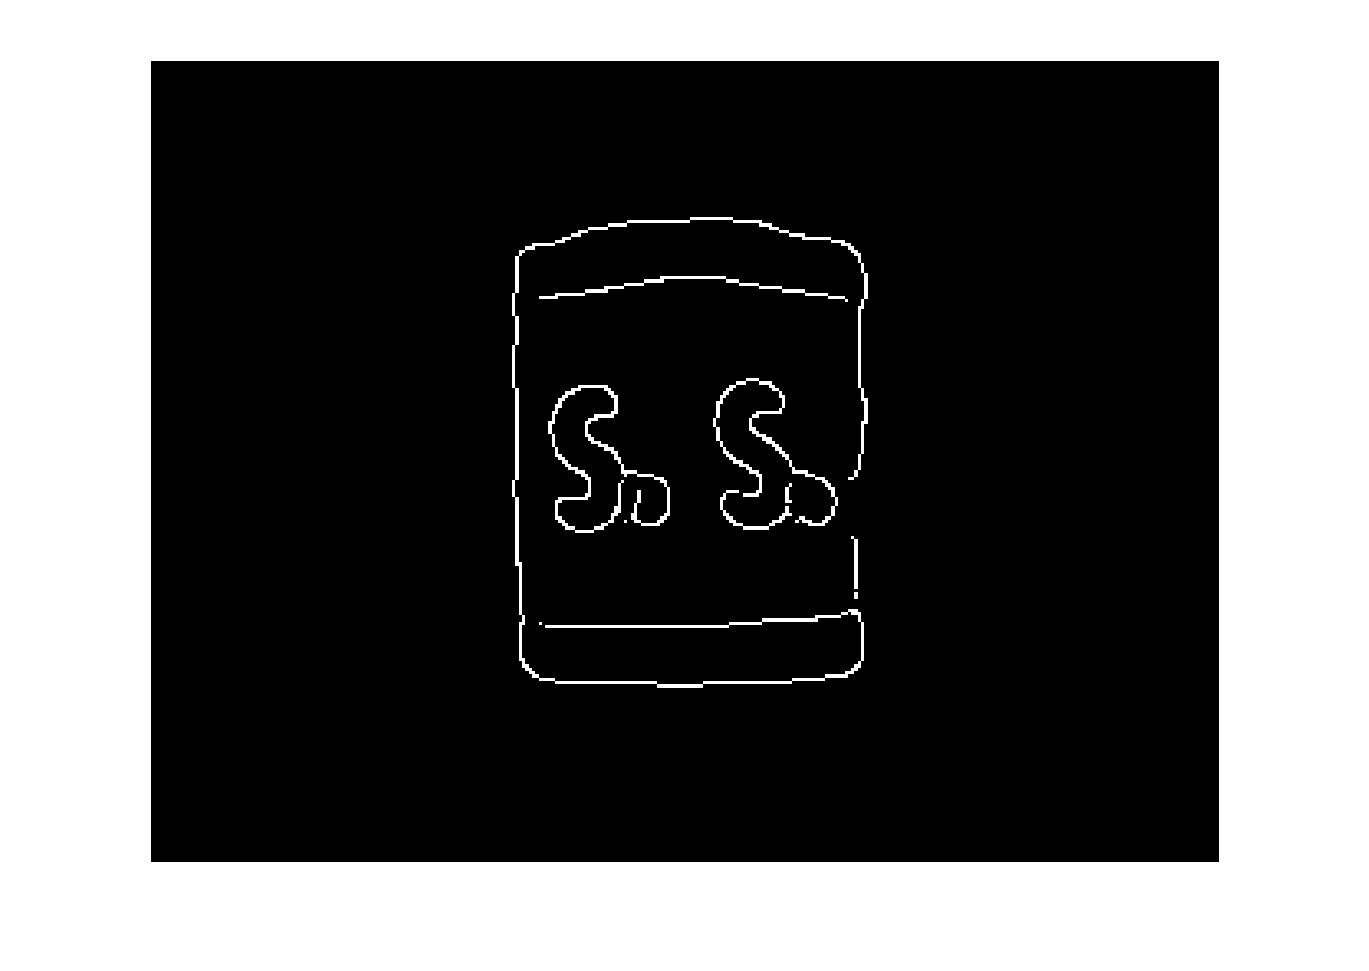
\includegraphics[width=0.5\textwidth]{figs/extracted_edge_mask}
  \caption{Extracted edges for ICP alignment}
  \label{fig:extracted_edge_mask}
\end{figure}

While in the assignment it was suggested to use
weighted transformation matrices we did not use that.
Utilising transformation from full point set of 
the box produced the same results as
transformation matrices that used points from 
the edges. That can be seen in figures 
\ref{fig:depth_points_after_edge_point_icp_alignment_ok}
and
\ref{fig:depth_points_after_full_point_icp_alignment_ok}.

\begin{figure}[h!]
    \centering
      \subfigure[Edge points before ICP alignment - top view]{
        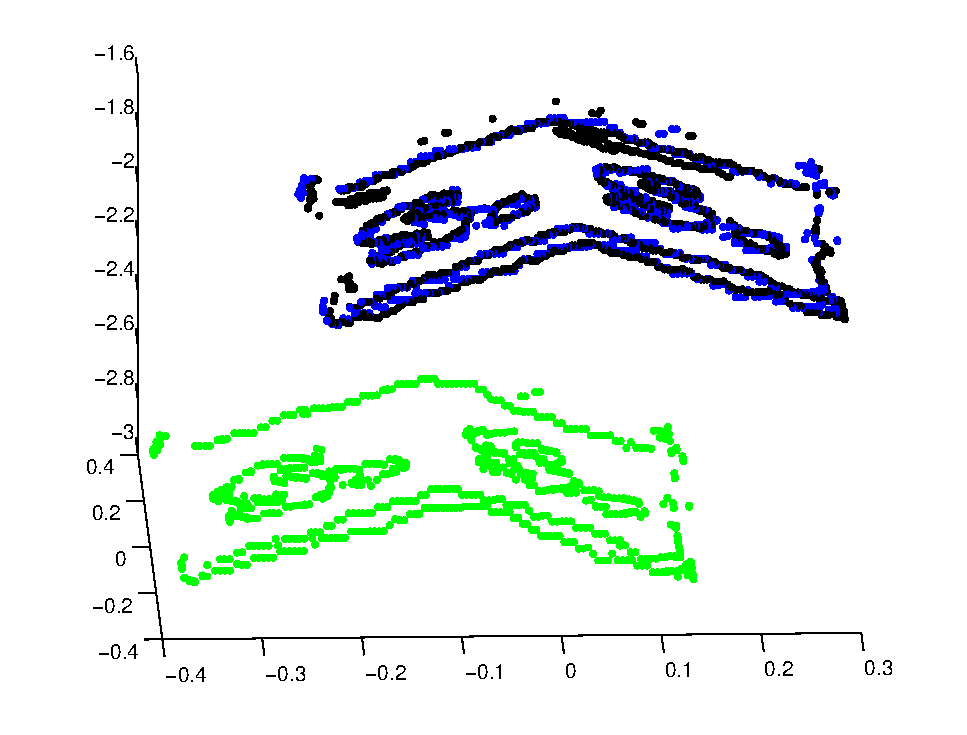
\includegraphics[width=0.4\linewidth]{figs/icp_before_alignment_from_side}
        \label{fig:icp_before_alignment_from_side}
      }
      \subfigure[Edge points before ICP alignment - side view]{
        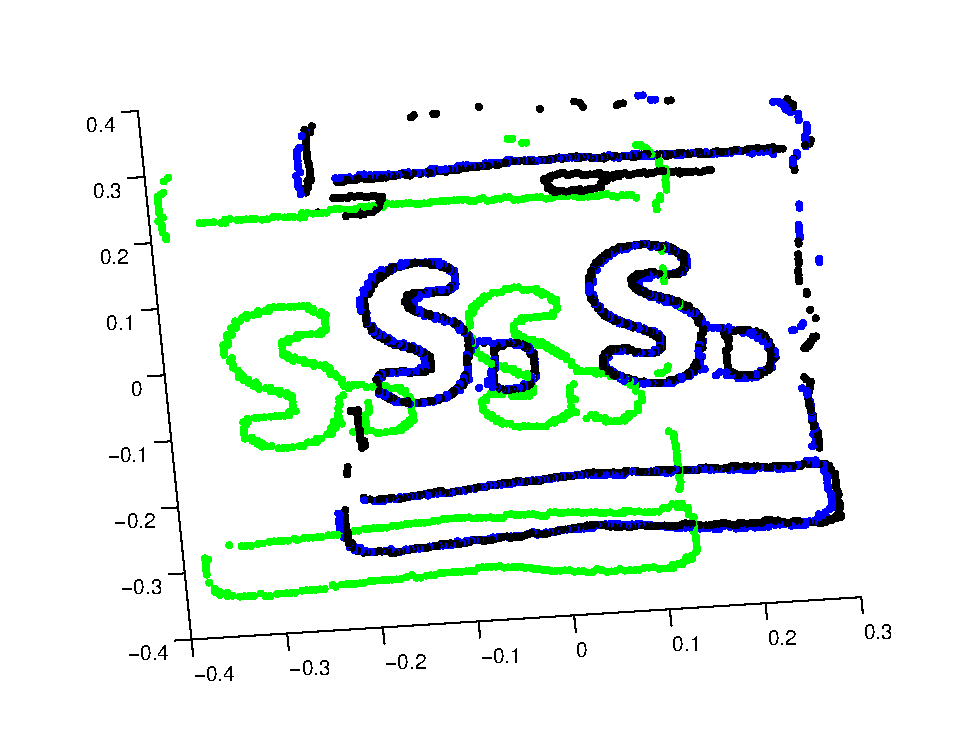
\includegraphics[width=0.4\linewidth]{figs/icp_before_alignment_from_top}
        \label{fig:icp_before_alignment_from_top}
      }
      \quad
      \subfigure[Extracted edge points aligned with foundation frame points]{
        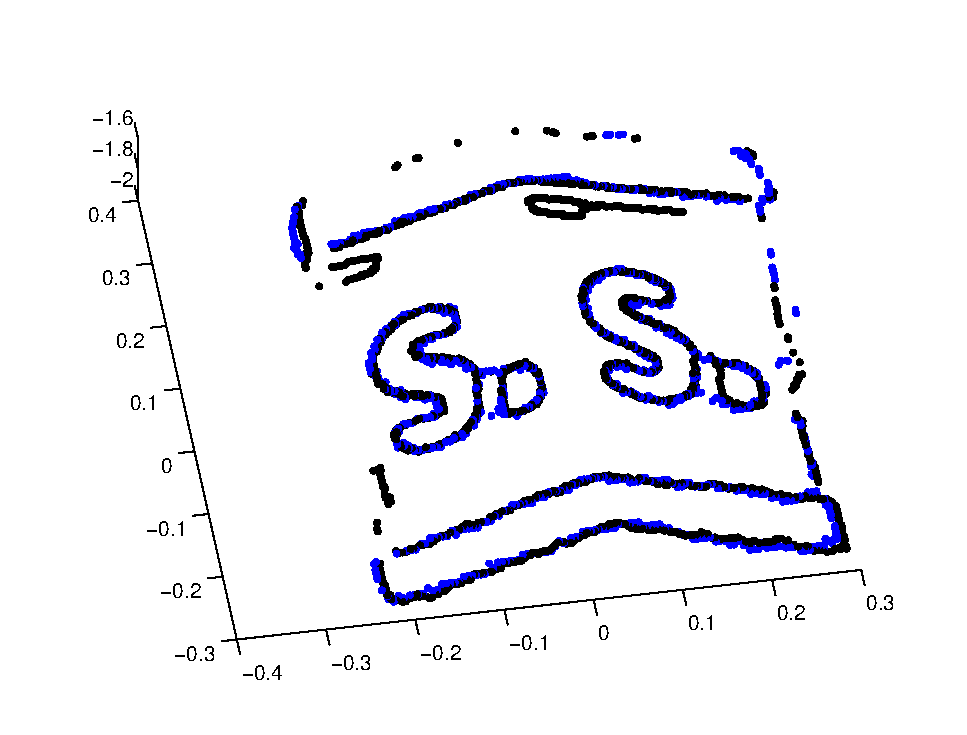
\includegraphics[width=0.4\linewidth]{figs/icp_point_alignment_example}
        \label{fig:icp_point_alignment_example}
      }
      \caption{ICP alignment examples}
\end{figure}

\begin{figure}[h!]
    \centering
      \subfigure[Depth point alignment using ICP transformations estimated only with edge points]{
        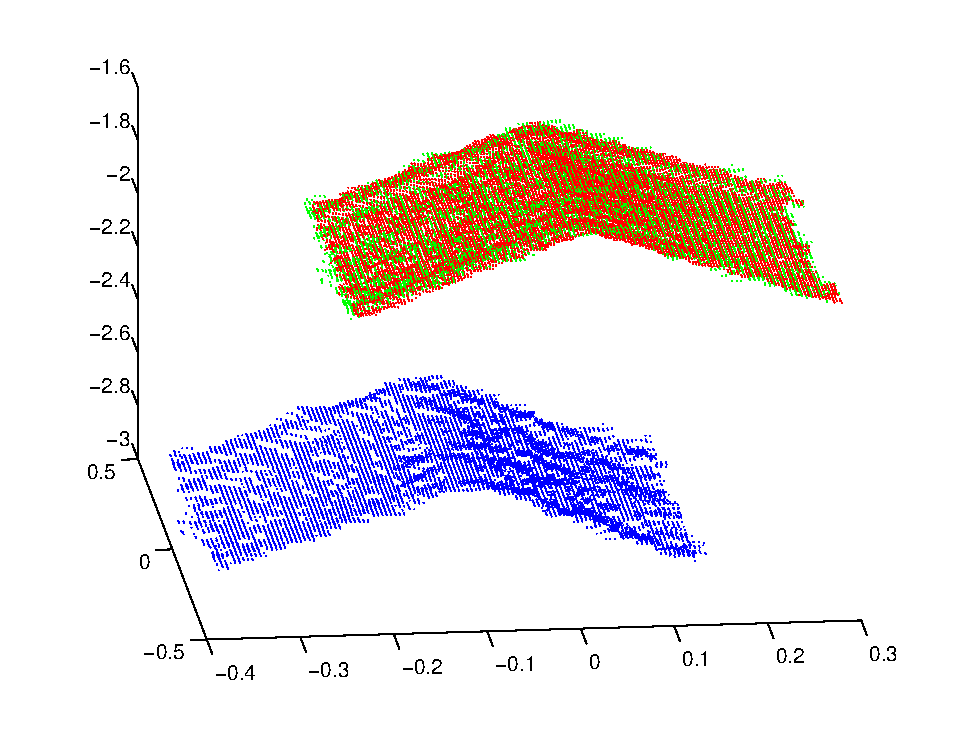
\includegraphics[width=0.4\linewidth]{figs/depth_points_after_edge_point_icp_alignment_ok}
        \label{fig:depth_points_after_edge_point_icp_alignment_ok}
      }
      \subfigure[Depth point alignment using ICP transformations estimated with 
      weighted edge points and full point set]{
        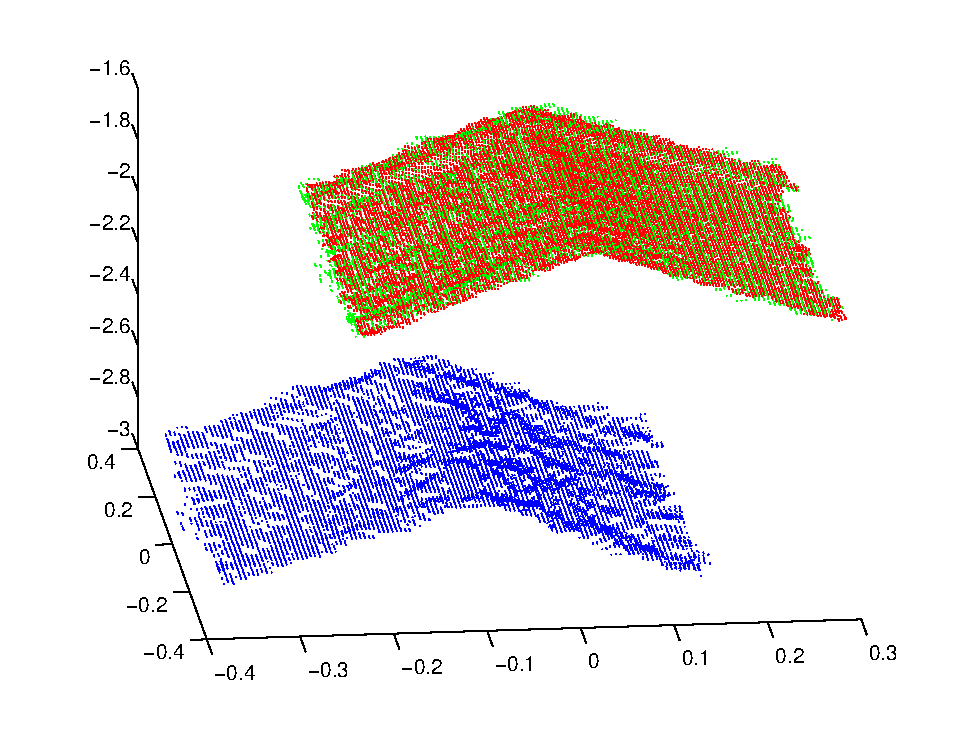
\includegraphics[width=0.4\linewidth]{figs/depth_points_after_full_point_icp_alignment_ok}
        \label{fig:depth_points_after_full_point_icp_alignment_ok}
      }
      \caption{Alignment of entire point dataset for the box. Red points are depth points from
      foundation frame, blue ones are from current frame for alignment and green ones (overlapping with red)
      are blue points after applying transformations estimated with ICP}
\end{figure}
\subsection{Plane fitting}
For plane extraction we chose to implement modified K-means algorithm.
It uses plane's normal vector $\vec{n}$  and data point $ (x,y,z) $
dot product as a distance measure. In maximization step it refits
plane on assigned data points for each plane
 using SVD (as given in "fitplane.m"
algorithm"). Code can be found in appendix \ref{apen:code_in}.

This approach easily allowed to fit data points to any of number of
planes that was required though it is prone (as regular K-mean is)
to initialization. To cope with this, thresholds were introduced
to find cases when initialization was definitely wrong.


\begin{figure}[h!]
    \centering
      \subfigure[Fitted planes]{
        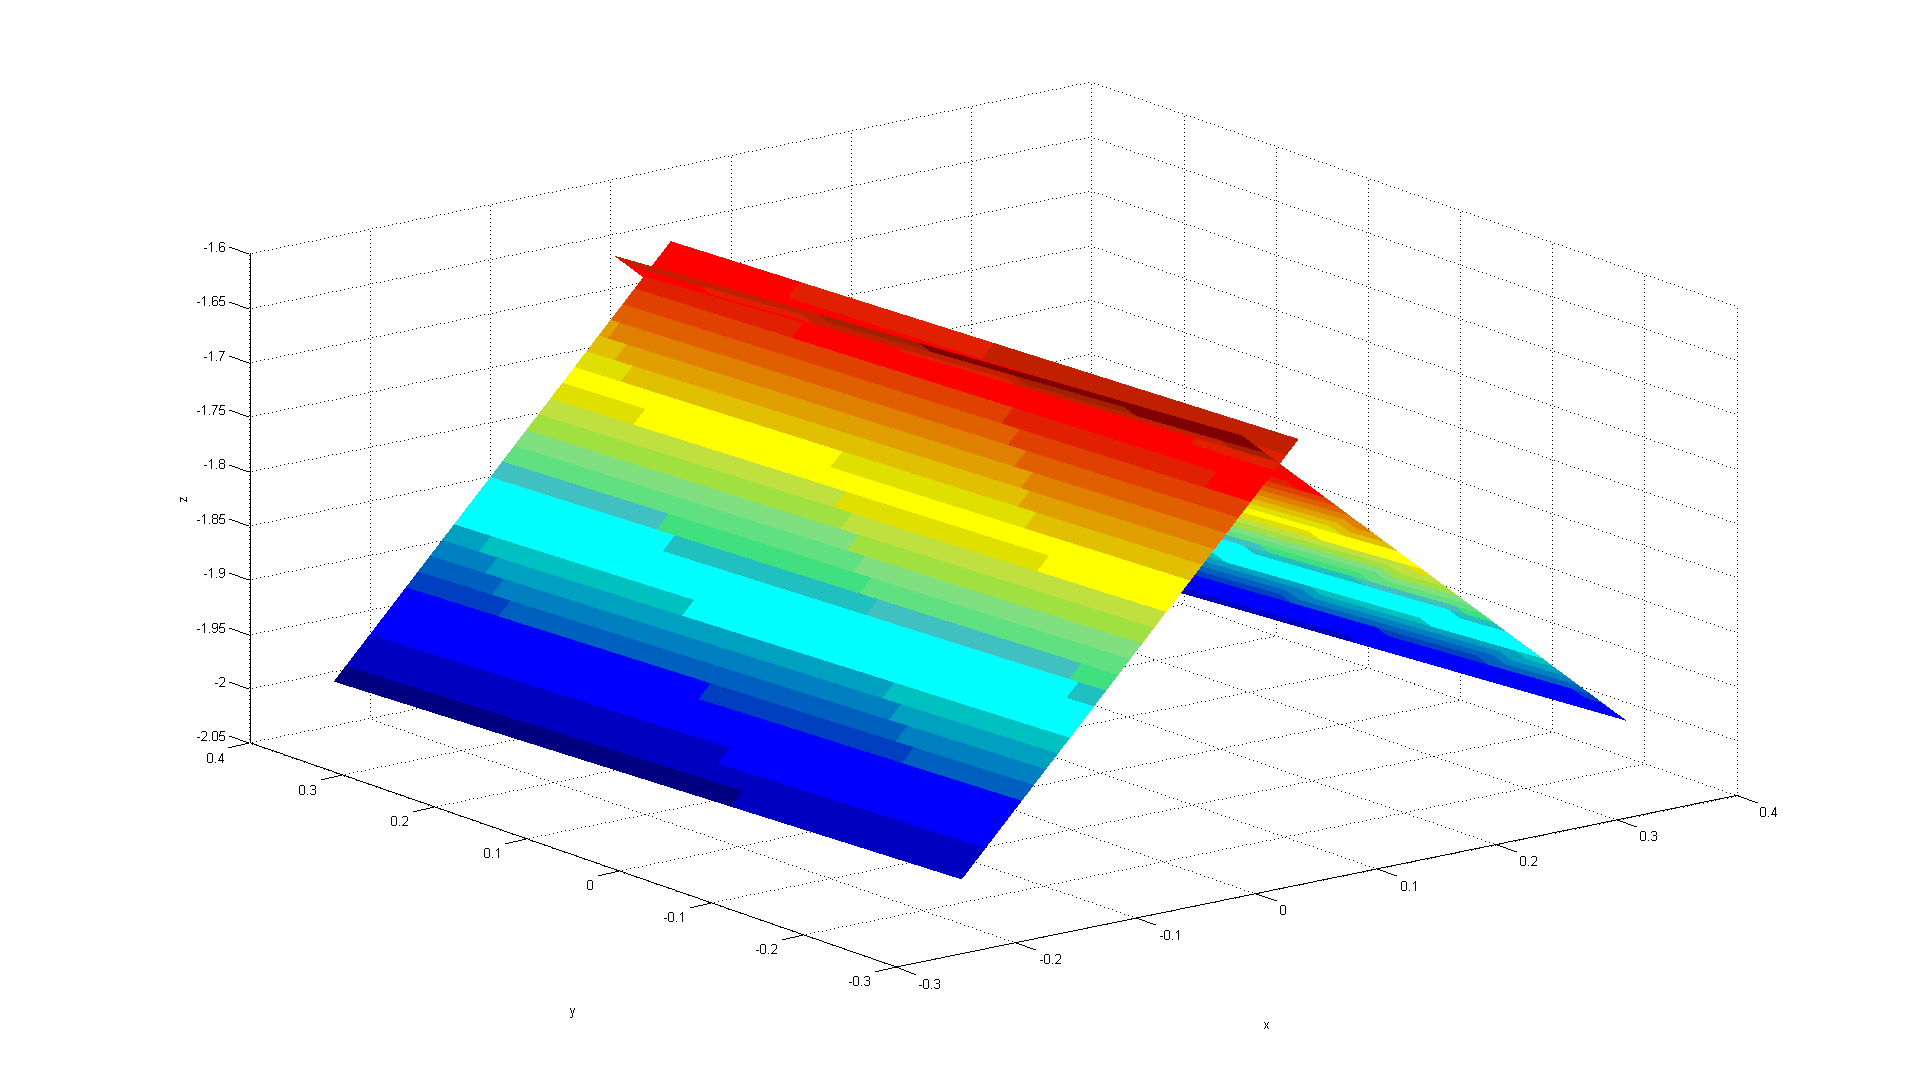
\includegraphics[width=0.4\linewidth]{figs/fitted_planes_without_points}
        \label{fig:fitted_planes_without_points}
      }
      \subfigure[Fitted planes together with final combined depth points]{
        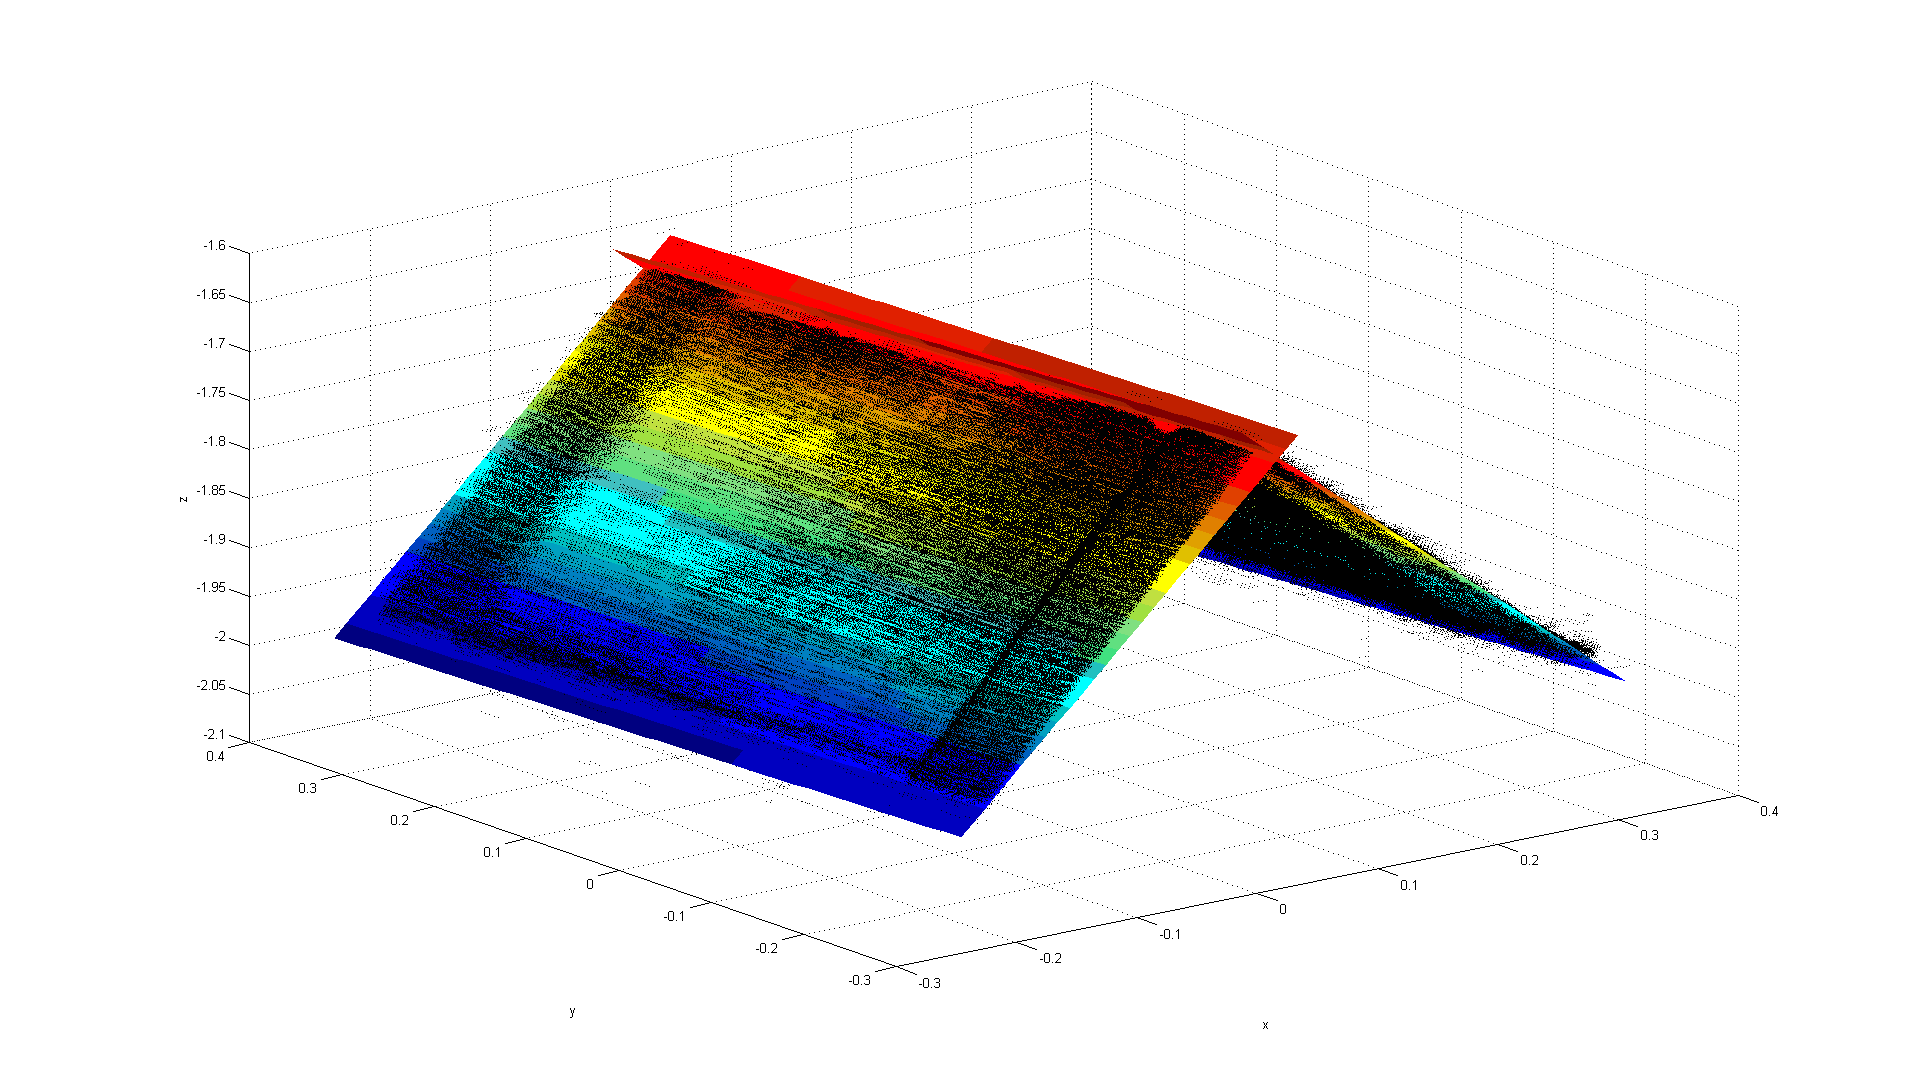
\includegraphics[width=0.4\linewidth]{figs/fitted_planes_with_points}
        \label{fig:fitted_planes_with_points}
      }
      \caption{Merged depth points shown together with fitted planes.}
\end{figure}
\section{Results}

\subsection{Dataset merging}

\subsection{Alignment accuracy}
\begin{figure}[h!]
  \centering
  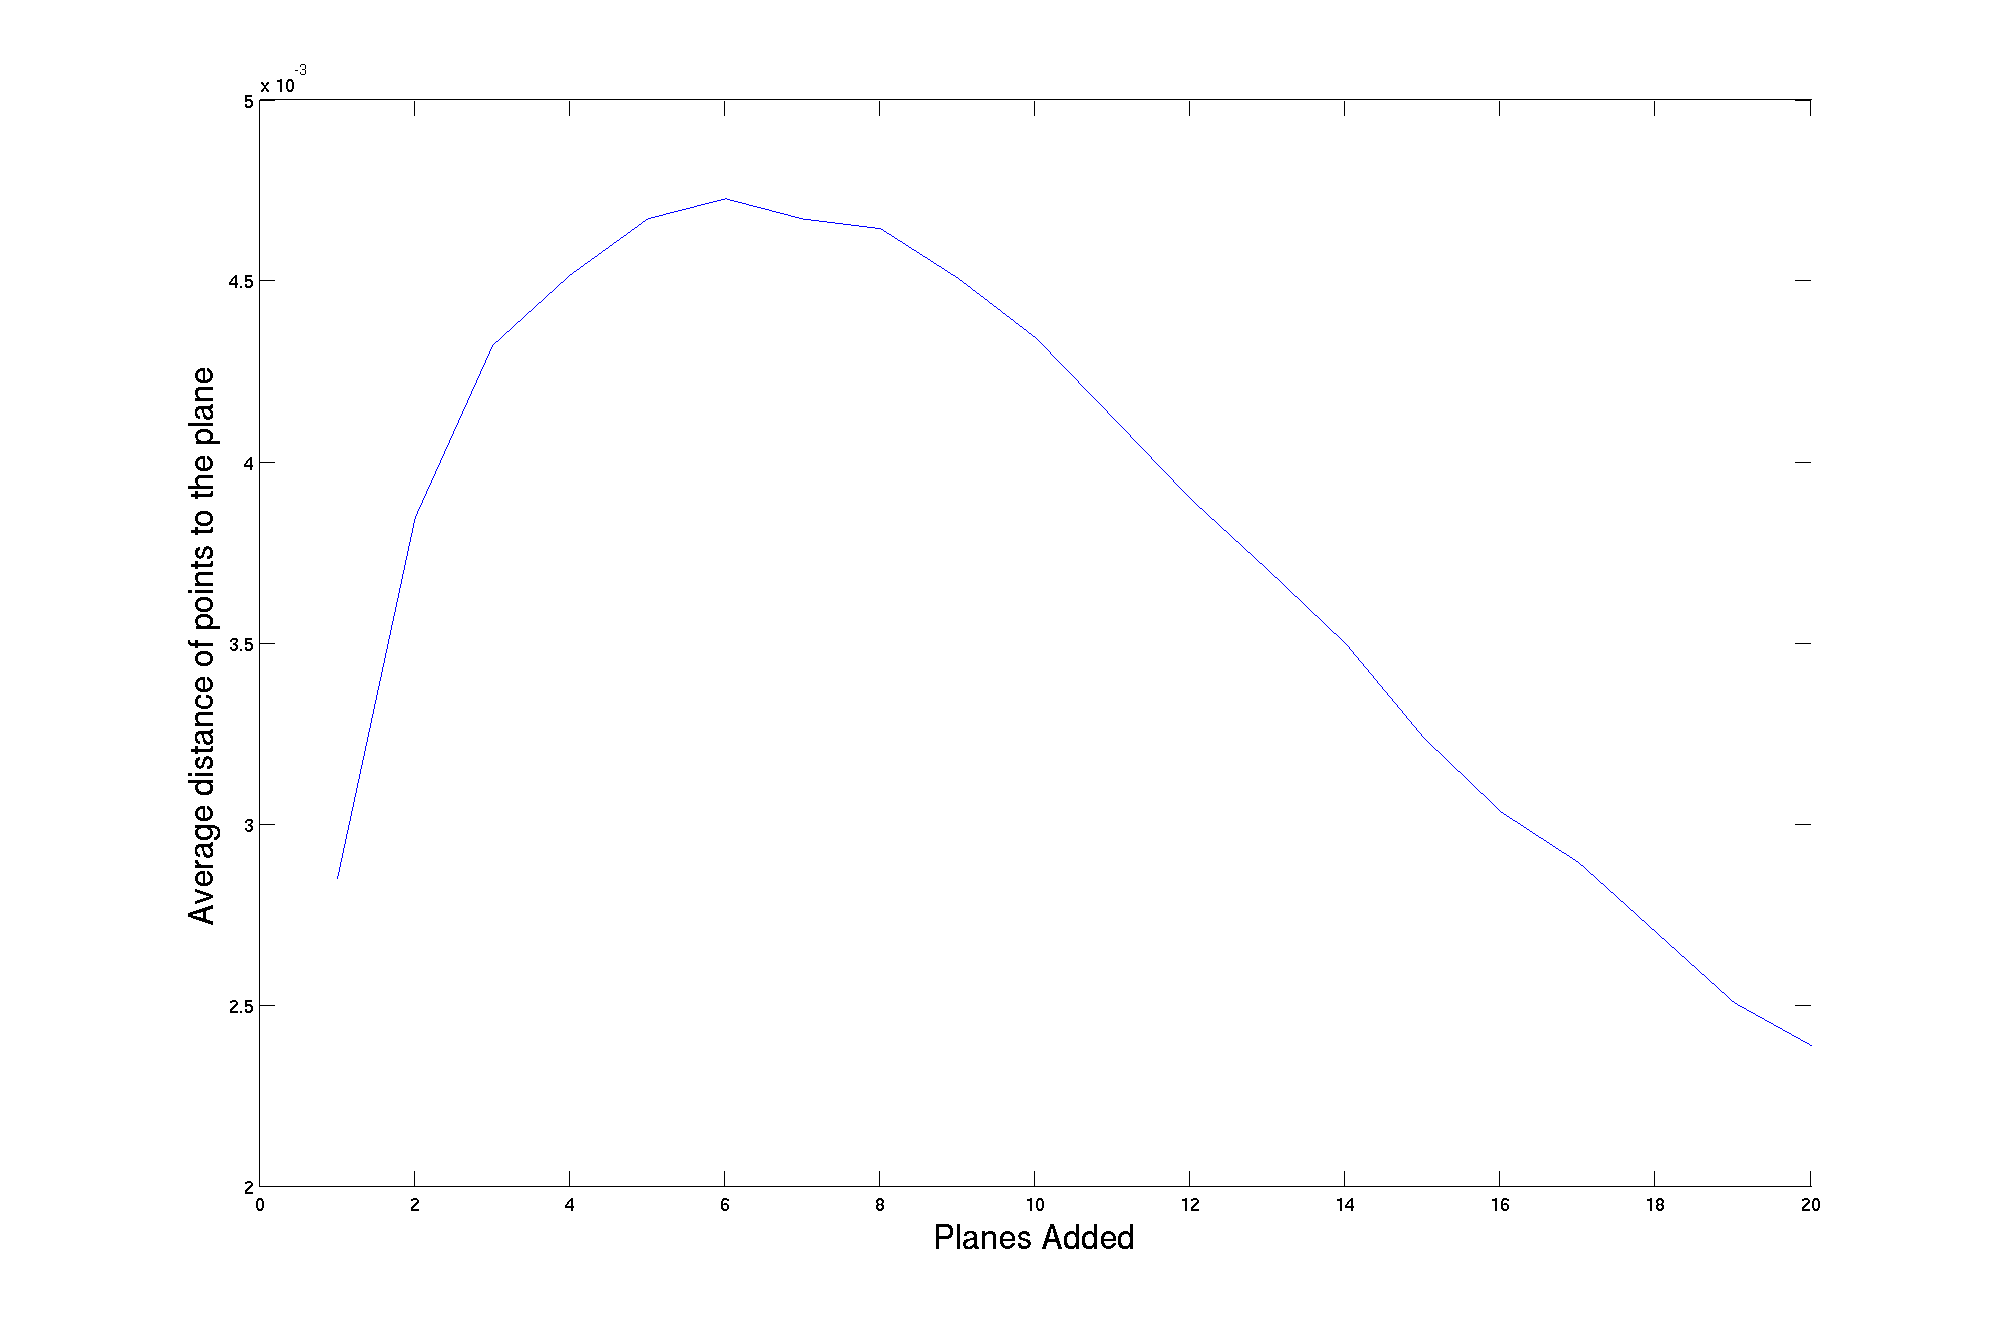
\includegraphics[width=0.5\textwidth]{figs/plane_angle_error_versus_foundation_plane}
  \caption{Dependency of frames combinedd and absolute mean distance of every point in "S." region to the plane}
  \label{fig:plane_angle_error_versus_foundation_plane}
\end{figure}
\subsection{Plane fitting}

\section{Discussion}
ICP and plane fitting algorithms in most cases 
worked without problems. K-means sometimes suffered
from poor initialization but that is easy to 
fix giving just a few checks of total
absolute error. The trickiest part is initial box
region detection. Finetuning color thresholds is tedious
process and always captures some artefacts around the box
that might have impact in later stages.

One of possible techniques to try for box detection
would be a probabilistic modelling - it might be possible
to detect background from whole series of frames
and then use it on each frame individually. 
We haven't tried this and just sticked with
easy to implement approach that works good enough.

\begin{thebibliography}{9}
  
\bibitem{lecture_code}
  ADVANCED VISION - TASK 4 MATLAB CODE
  \url{http://www.inf.ed.ac.uk/teaching/courses/av/MATLAB/TASK4/} 
  
\end{thebibliography}

\appendix


\newpage



\newpage
\section{Code}
\label{apen:code_in}

%\lstinputlisting[caption=assgn\_tracking.m, language=Matlab]{../assgn_tracking.m}




\end{document}
